\documentclass{article}
\usepackage{enumerate}
\usepackage{amsmath}
\usepackage{amssymb}
\usepackage{graphicx}
\usepackage{subfigure}
\usepackage{geometry}
\usepackage{caption}
\usepackage{indentfirst}
\usepackage{tikz}
\usetikzlibrary{circuits.logic.US}
\usetikzlibrary{arrows.meta}
\usetikzlibrary{calc}
\geometry{left=3.0cm,right=3.0cm,top=3.0cm,bottom=3.0cm}
\renewcommand{\thesection}{Problem \arabic{section}.}
\newcommand{\unit}[1]{{\rm\,#1}}
\title{VE270 Homework 10}
\author{Liu Yihao 515370910207}
\date{}

\begin{document}
\maketitle

\section{}
\begin{enumerate}[(a)]
\item
The truth table is 

\begin{center}
\begin{tabular}{ccccc|cccccccc}
$s_{2}$ & $s_{1}$ & $s_{0}$ & $B$ & $S$ & $n_{2}$ & $n_{1}$ & $n_{0}$ & $L$ & $Dreg\_clr$ & $Dreg\_ld$ & $Dctr\_clr$ & $Dctr\_ld$ \\
\hline
0 & 0 & 0 & 0 & 0 & 0 & 0 & 1 & 0 & 1 & 0 & 0 & 0 \\
0 & 0 & 0 & 0 & 1 & 0 & 0 & 1 & 0 & 1 & 0 & 0 & 0 \\
0 & 0 & 0 & 1 & 0 & 0 & 0 & 1 & 0 & 1 & 0 & 0 & 0 \\
0 & 0 & 0 & 1 & 1 & 0 & 0 & 1 & 0 & 1 & 0 & 0 & 0 \\
0 & 0 & 1 & 0 & 0 & 0 & 1 & 0 & 0 & 0 & 0 & 1 & 0 \\
0 & 0 & 1 & 0 & 1 & 0 & 1 & 0 & 0 & 0 & 0 & 1 & 0 \\
0 & 0 & 1 & 1 & 0 & 0 & 0 & 1 & 0 & 0 & 0 & 1 & 0 \\
0 & 0 & 1 & 1 & 1 & 0 & 0 & 1 & 0 & 0 & 0 & 1 & 0 \\
0 & 1 & 0 & 0 & 0 & 0 & 1 & 1 & 1 & 0 & 0 & 0 & 0 \\
0 & 1 & 0 & 0 & 1 & 0 & 1 & 1 & 1 & 0 & 0 & 0 & 0 \\
0 & 1 & 0 & 1 & 0 & 0 & 1 & 1 & 1 & 0 & 0 & 0 & 0 \\
0 & 1 & 0 & 1 & 1 & 0 & 1 & 1 & 1 & 0 & 0 & 0 & 0 \\
0 & 1 & 1 & 0 & 0 & 0 & 1 & 1 & 0 & 0 & 0 & 0 & 1 \\
0 & 1 & 1 & 0 & 1 & 1 & 0 & 0 & 0 & 0 & 0 & 0 & 1 \\
0 & 1 & 1 & 1 & 0 & 0 & 1 & 1 & 0 & 0 & 0 & 0 & 1 \\
0 & 1 & 1 & 1 & 1 & 1 & 0 & 0 & 0 & 0 & 0 & 0 & 1 \\
1 & 0 & 0 & 0 & 0 & 0 & 0 & 1 & 0 & 0 & 1 & 0 & 0 \\
1 & 0 & 0 & 0 & 1 & 0 & 0 & 1 & 0 & 0 & 1 & 0 & 0 \\
1 & 0 & 0 & 1 & 0 & 0 & 0 & 1 & 0 & 0 & 1 & 0 & 0 \\
1 & 0 & 0 & 1 & 1 & 0 & 0 & 1 & 0 & 0 & 1 & 0 & 0 \\
1 & 0 & 1 & 0 & 0 & X & X & X & X & X & X & X & X \\
1 & 0 & 1 & 0 & 1 & X & X & X & X & X & X & X & X \\
1 & 0 & 1 & 1 & 0 & X & X & X & X & X & X & X & X \\
1 & 0 & 1 & 1 & 1 & X & X & X & X & X & X & X & X \\
1 & 1 & 0 & 0 & 0 & X & X & X & X & X & X & X & X \\
1 & 1 & 0 & 0 & 1 & X & X & X & X & X & X & X & X \\
1 & 1 & 0 & 1 & 0 & X & X & X & X & X & X & X & X \\
1 & 1 & 0 & 1 & 1 & X & X & X & X & X & X & X & X \\
1 & 1 & 1 & 0 & 0 & X & X & X & X & X & X & X & X \\
1 & 1 & 1 & 0 & 1 & X & X & X & X & X & X & X & X \\
1 & 1 & 1 & 1 & 0 & X & X & X & X & X & X & X & X \\
1 & 1 & 1 & 1 & 1 & X & X & X & X & X & X & X & X \\
\end{tabular}
\end{center}

The euqations are 

$$n_{2}=s_{1}s_{0}S$$
$$n_{1}=s_{1}'s_{0}B'+s_{1}s_{0}'+s_{1}S'$$
$$n_{0}=s_{1}'B+s_{1}S'+s_{0}'$$
$$L=s_{1}s_{0}'$$
$$Dreg\_clr=s_{2}'s_{1}'s_{0}'$$
$$Dreg\_ld=s_{2}$$
$$Dctr\_clr=s_{1}'s_{0}$$
$$Dctr\_ld=s_{1}s_{0}$$


The schematics is 

\begin{center}
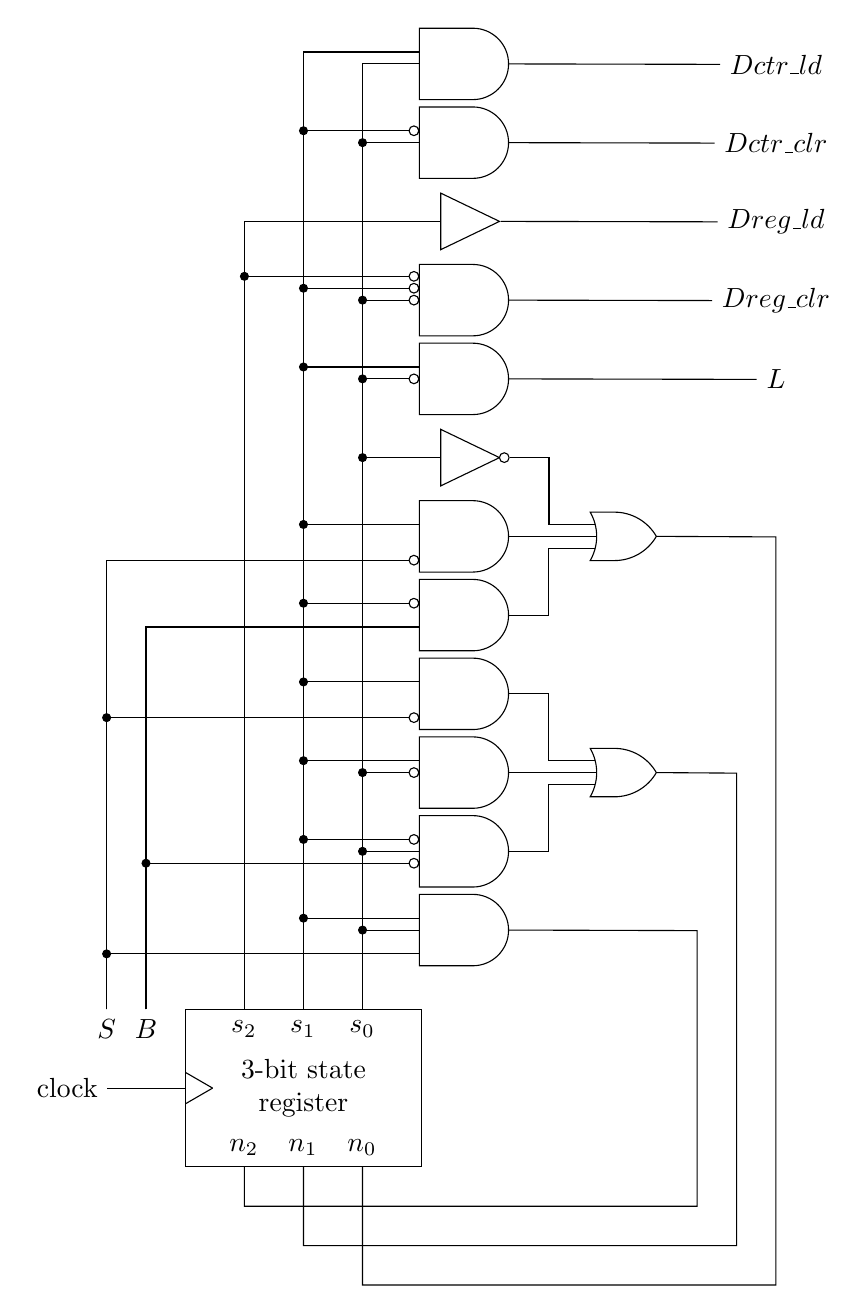
\begin{tikzpicture}[circuit logic US]
\draw (0,0) node (r) [shape=rectangle,draw,minimum height=2cm,minimum width=3cm,text width=2cm,align=center] {3-bit state register};
\draw (-3,0) node (clock) {clock};\draw (clock) -- (r.west);\draw (r) ++(left:11.54mm) -- ++($(left:3.46mm)+(down:2mm)$);
\draw (r) ++(left:11.54mm) -- ++($(left:3.46mm)+(up:2mm)$);
\draw (r.west) ++(up:7.5mm) ++(right:7.500000mm) node {$s_2$};
\draw (r.west) ++(down:7.5mm) ++(right:7.500000mm) node {$n_2$};
\draw (r.west) ++(up:7.5mm) ++(right:15.000000mm) node {$s_1$};
\draw (r.west) ++(down:7.5mm) ++(right:15.000000mm) node {$n_1$};
\draw (r.west) ++(up:7.5mm) ++(right:22.500000mm) node {$s_0$};
\draw (r.west) ++(down:7.5mm) ++(right:22.500000mm) node {$n_0$};
\draw (-2.000000,0.750000) node {$B$};
\draw (-2.500000,0.750000) node {$S$};
\draw (r.north) ++(up:1.000000cm) ++(right:2cm) node (and1) [and gate,inputs=nnnnn] {};
\draw (0.000000,1.000000) |- (and1.input 2) ;
\draw (0.750000,1.000000) |- (and1.input 3) ;
\draw (-2.500000,1.000000) |- (and1.input 5) ;
\draw (and1.output) -- (5.000000,2.000000) -- (5.000000,-1.500000) -| (-0.750000,-1);
\draw (r.north) ++(up:2.000000cm) ++(right:2cm) node (and2) [and gate,inputs=ninin] {};
\draw (0.000000,1.000000) |- (and2.input 2) ;
\draw (0.750000,1.000000) |- (and2.input 3) ;
\draw (-2.000000,1.000000) |- (and2.input 4) ;
\draw (and1.input 2) ;
\pgfgetlastxy{\x}{\y};
\filldraw (0.000000,\y) circle [radius=0.5mm];
\draw (and1.input 3) ;
\pgfgetlastxy{\x}{\y};
\filldraw (0.750000,\y) circle [radius=0.5mm];
\draw (r.north) ++(up:3.000000cm) ++(right:2cm) node (and3) [and gate,inputs=nninn] {};
\draw (0.000000,1.000000) |- (and3.input 2) ;
\draw (0.750000,1.000000) |- (and3.input 3) ;
\draw (and2.input 2) ;
\pgfgetlastxy{\x}{\y};
\filldraw (0.000000,\y) circle [radius=0.5mm];
\draw (and2.input 3) ;
\pgfgetlastxy{\x}{\y};
\filldraw (0.750000,\y) circle [radius=0.5mm];
\draw (r.north) ++(up:4.000000cm) ++(right:2cm) node (and4) [and gate,inputs=nnnni] {};
\draw (0.000000,1.000000) |- (and4.input 2) ;
\draw (-2.500000,1.000000) |- (and4.input 5) ;
\draw (and3.input 2) ;
\pgfgetlastxy{\x}{\y};
\filldraw (0.000000,\y) circle [radius=0.5mm];
\draw (and1.input 5) ;
\pgfgetlastxy{\x}{\y};
\filldraw (-2.500000,\y) circle [radius=0.5mm];
\draw (r.north) ++(up:3.000000cm) ++(right:4cm) node (or2) [or gate,inputs=nnn] {};
\draw (and2.output) -- ++(right:0.500000cm) |- (or2.input 3);
\draw (and3.output) -- ++(right:0.000000cm) |- (or2.input 2);
\draw (and4.output) -- ++(right:0.500000cm) |- (or2.input 1);
\draw (or2.output) -- (5.500000,4.000000) -- (5.500000,-2.000000) -| (0.000000,-1);
\draw (r.north) ++(up:5.000000cm) ++(right:2cm) node (and5) [and gate,inputs=ninnn] {};
\draw (0.000000,1.000000) |- (and5.input 2) ;
\draw (-2.000000,1.000000) |- (and5.input 4) ;
\draw (and4.input 2) ;
\pgfgetlastxy{\x}{\y};
\filldraw (0.000000,\y) circle [radius=0.5mm];
\draw (and2.input 4) ;
\pgfgetlastxy{\x}{\y};
\filldraw (-2.000000,\y) circle [radius=0.5mm];
\draw (r.north) ++(up:6.000000cm) ++(right:2cm) node (and6) [and gate,inputs=nnnni] {};
\draw (0.000000,1.000000) |- (and6.input 2) ;
\draw (-2.500000,1.000000) |- (and6.input 5) ;
\draw (and5.input 2) ;
\pgfgetlastxy{\x}{\y};
\filldraw (0.000000,\y) circle [radius=0.5mm];
\draw (and4.input 5) ;
\pgfgetlastxy{\x}{\y};
\filldraw (-2.500000,\y) circle [radius=0.5mm];
\draw (r.north) ++(up:7.000000cm) ++(right:2cm) node (and7) [not gate] {};
\draw (0.750000,1.000000) |- (and7.input) ;
\draw (and3.input 3) ;
\pgfgetlastxy{\x}{\y};
\filldraw (0.750000,\y) circle [radius=0.5mm];
\draw (r.north) ++(up:6.000000cm) ++(right:4cm) node (or3) [or gate,inputs=nnn] {};
\draw (and5.output) -- ++(right:0.500000cm) |- (or3.input 3);
\draw (and6.output) -- ++(right:0.000000cm) |- (or3.input 2);
\draw (and7.output) -- ++(right:0.500000cm) |- (or3.input 1);
\draw (or3.output) -- (6.000000,7.000000) -- (6.000000,-2.500000) -| (0.750000,-1);
\draw (r.north) ++(up:8.000000cm) ++(right:2cm) node (and8) [and gate,inputs=nninn] {};
\draw (0.000000,1.000000) |- (and8.input 2) ;
\draw (0.750000,1.000000) |- (and8.input 3) ;
\draw (and6.input 2) ;
\pgfgetlastxy{\x}{\y};
\filldraw (0.000000,\y) circle [radius=0.5mm];
\draw (and7.input) ;
\pgfgetlastxy{\x}{\y};
\filldraw (0.750000,\y) circle [radius=0.5mm];
\draw (6,9.000000) node (out1) {$L$};
\draw (and8.output) -- (out1);
\draw (r.north) ++(up:9.000000cm) ++(right:2cm) node (and9) [and gate,inputs=iiinn] {};
\draw (-0.750000,1.000000) |- (and9.input 1) ;
\draw (0.000000,1.000000) |- (and9.input 2) ;
\draw (0.750000,1.000000) |- (and9.input 3) ;
\draw (and8.input 2) ;
\pgfgetlastxy{\x}{\y};
\filldraw (0.000000,\y) circle [radius=0.5mm];
\draw (and8.input 3) ;
\pgfgetlastxy{\x}{\y};
\filldraw (0.750000,\y) circle [radius=0.5mm];
\draw (6,10.000000) node (out2) {$Dreg\_clr$};
\draw (and9.output) -- (out2);
\draw (r.north) ++(up:10.000000cm) ++(right:2cm) node (and10) [buffer gate] {};
\draw (-0.750000,1.000000) |- (and10.input) ;
\draw (and9.input 1) ;
\pgfgetlastxy{\x}{\y};
\filldraw (-0.750000,\y) circle [radius=0.5mm];
\draw (6,11.000000) node (out3) {$Dreg\_ld$};
\draw (and10.output) -- (out3);
\draw (r.north) ++(up:11.000000cm) ++(right:2cm) node (and11) [and gate,inputs=ninnn] {};
\draw (0.000000,1.000000) |- (and11.input 2) ;
\draw (0.750000,1.000000) |- (and11.input 3) ;
\draw (and9.input 2) ;
\pgfgetlastxy{\x}{\y};
\filldraw (0.000000,\y) circle [radius=0.5mm];
\draw (and9.input 3) ;
\pgfgetlastxy{\x}{\y};
\filldraw (0.750000,\y) circle [radius=0.5mm];
\draw (6,12.000000) node (out4) {$Dctr\_clr$};
\draw (and11.output) -- (out4);
\draw (r.north) ++(up:12.000000cm) ++(right:2cm) node (and12) [and gate,inputs=nnnnn] {};
\draw (0.000000,1.000000) |- (and12.input 2) ;
\draw (0.750000,1.000000) |- (and12.input 3) ;
\draw (and11.input 2) ;
\pgfgetlastxy{\x}{\y};
\filldraw (0.000000,\y) circle [radius=0.5mm];
\draw (and11.input 3) ;
\pgfgetlastxy{\x}{\y};
\filldraw (0.750000,\y) circle [radius=0.5mm];
\draw (6,13.000000) node (out5) {$Dctr\_ld$};
\draw (and12.output) -- (out5);
\end{tikzpicture}
\end{center}

\item
The critical path is the 16-bit up counter, so the delay is 5 ns.
\item
The maximum clock frequency is $1/5\unit{ns}=200\unit{MHz}$.
\end{enumerate}

\section{}
The SRAM block can have $2^{32}\times8=34359738368$ bits in maximum.

\section{}
The approximate number of SRAM bit storage cells is $\lfloor 10000000/6 \rfloor=1666666$.

\section{}
SRAM cells have 6 transistors and is faster but DRAM cells have only 1 transistor and is slower. What's more, DRAM uses capacitor which discharges overtime so that it must be refreshed regularly, but SRAM needn't.

\section{}
EEPROMs are erased electronically, but flash memories can be erased simultaneously.

\section{}
Inputs: $S$ (1-bit), $P$ (1-bit), $R$ (1-bit), $D$ (8-bit)

Outputs: $Q$ (8-bit)

Local Registers: $S_0$ (1-bit), $P_0$ (1-bit), $s\_cnt$ (16-bit), $p\_cnt$ (16-bit)

Memory: mem (10000x8 SRAM)

\begin{center}
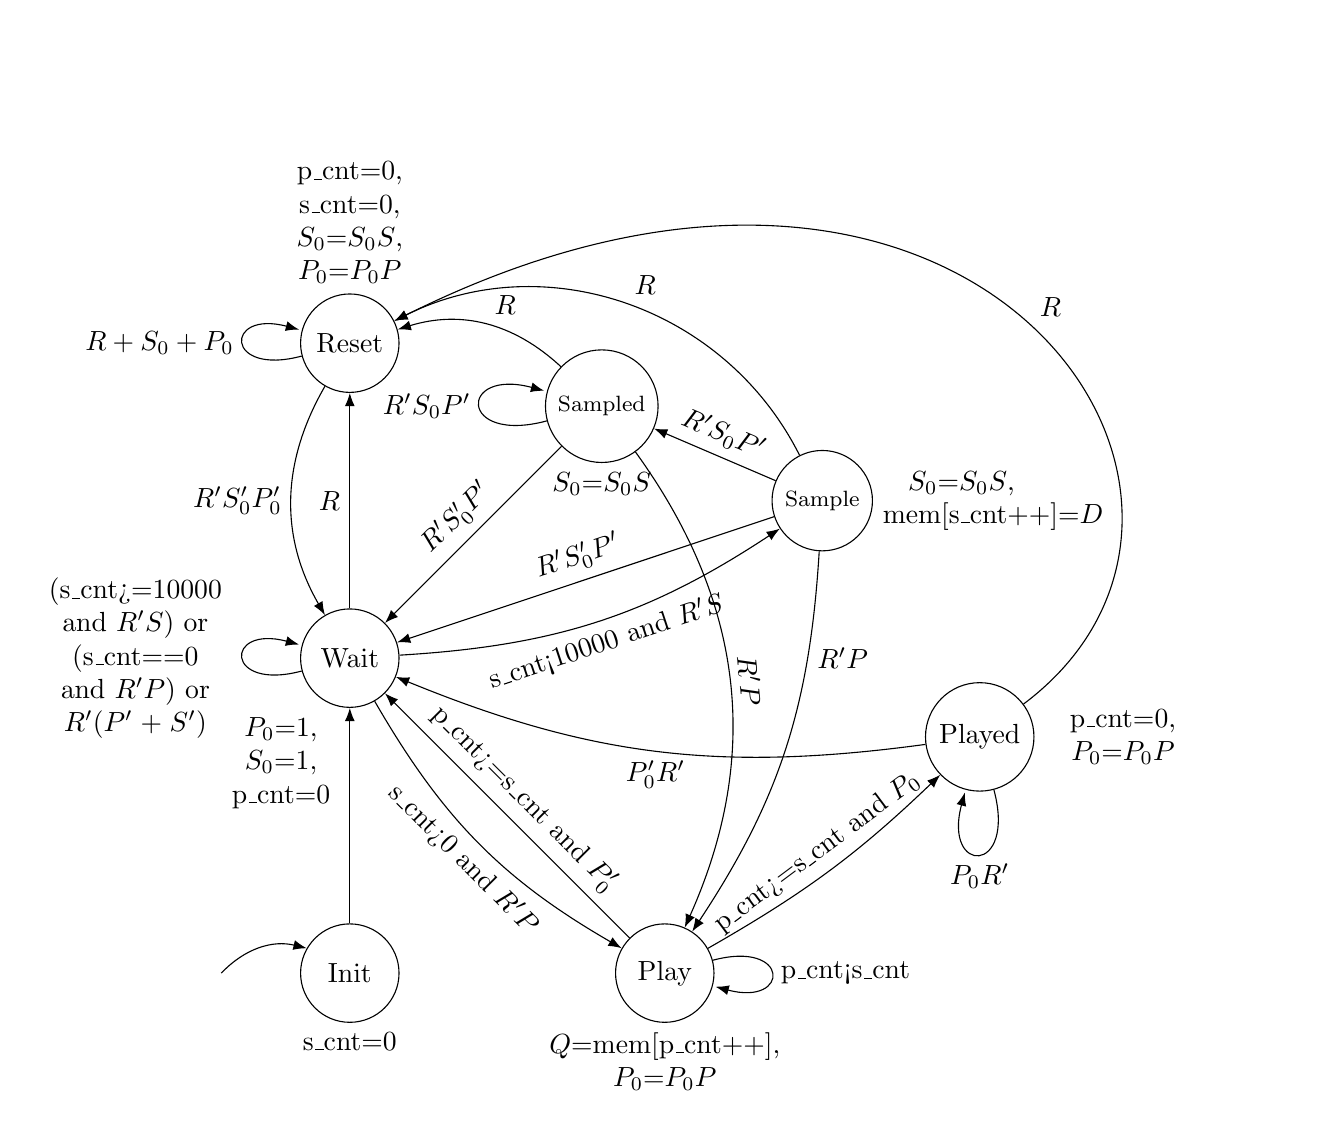
\begin{tikzpicture}[>/.tip={Latex}]
	\draw (0,-4) node (init) [draw,shape=circle,minimum size=1.25cm] {Init};
	\node [below,text width=1.5cm,align=center] at (init.south) {s\_cnt=0};

	\draw (0,0) node (wait) [draw,shape=circle,minimum size=1.25cm] {Wait};
	\node [below left,text width=1.5cm,align=center] at (wait.south) {$P_0$=1, $S_0$=1, p\_cnt=0};
	
	\draw (0,4) node (reset) [draw,shape=circle,minimum size=1.25cm] {Reset};
	\node [above,text width=2cm,align=center] at (reset.north) {p\_cnt=0, s\_cnt=0, $S_0$=$S_0S$, $P_0$=$P_0P$};	
	
	\draw (6,2) node (sample) [draw,shape=circle,minimum size=1.25cm] {\footnotesize Sample};
	\node [right,text width=2cm,align=center] at (sample.east) {$S_0$=$S_0S$, mem[s\_cnt++]=$D$};
	
	\draw (3.2,3.2) node (sampled) [draw,shape=circle,minimum size=1.25cm] {\footnotesize Sampled};
	\node [below,text width=2cm,align=center] at (sampled.south) {$S_0$=$S_0S$};
	
	\draw (4,-4) node (play) [draw,shape=circle,minimum size=1.25cm] {Play};
	\node [below,text width=3cm,align=center] at (play.south) {$Q$=mem[p\_cnt++], $P_0$=$P_0P$};
	
	\draw (8,-1) node (played) [draw,shape=circle,minimum size=1.25cm] {Played};
	\node [right,text width=2cm,align=center] at (played.east) {p\_cnt=0, $P_0$=$P_0P$};	
	
	\path[->] (init.west)++(left:1cm) edge [bend left=30] (init);
	\path[->] (init) edge (wait);
	\path[->] (wait) edge node [left] {$R$} (reset);
	\path[->] (reset) edge [bend right=30] node [left] {$R'S_0'P_0'$} (wait);
	\path[->] (wait) edge [loop left] node [text width=2.5cm,align=center] {(s\_cnt>=10000 and $R'S$) or (s\_cnt==0 and $R'P$) or $R'(P'+S')$} ();
	\path[->] (reset) edge [loop left] node {$R+S_0+P_0$} ();
	\path[->] (wait) edge [bend right=15] node [below,sloped] {s\_cnt>0 and $R'P$} (play);
	\path[->] (wait) edge [bend right=15] node [below,sloped] {s\_cnt<10000 and $R'S$} (sample);
	\path[->] (sample) edge node [above,sloped] {$R'S_0'P'$} (wait);
	\path[->] (play) edge [loop right] node {p\_cnt<s\_cnt} ();
	\path[->] (sample) edge node [above,sloped] {$R'S_0P'$} (sampled);
	\path[->] (play) edge [bend right=7] node [above,sloped] {p\_cnt>=s\_cnt and $P_0$} (played);
	\path[->] (play) edge node [above,sloped] {p\_cnt>=s\_cnt and $P_0'$} (wait);
	\path[->] (played) edge [loop below] node {$P_0R'$} ();
	\path[->] (played) edge [bend left=15] node [below] {$P_0'R'$} (wait);
	\draw[->] (played) .. controls (12,2) and (8,8) .. node [above right] {$R$} (reset);
	\path[->] (sample) edge [bend right=45] node [above right] {$R$} (reset);
	\path[->] (sample) edge [bend left=15] node [near start,right] {$R'P$} (play);
	\path[->] (sampled) edge [bend right=30] node [above right] {$R$} (reset);
	\path[->] (sampled) edge node [above,sloped] {$R'S_0'P'$} (wait);
	\path[->] (sampled) edge [loop left] node {$R'S_0P'$} ();
	\path[->] (sampled) edge [bend left=30] node [above,sloped] {$R'P$} (play);
\end{tikzpicture}
\end{center}

\section{}
\begin{center}
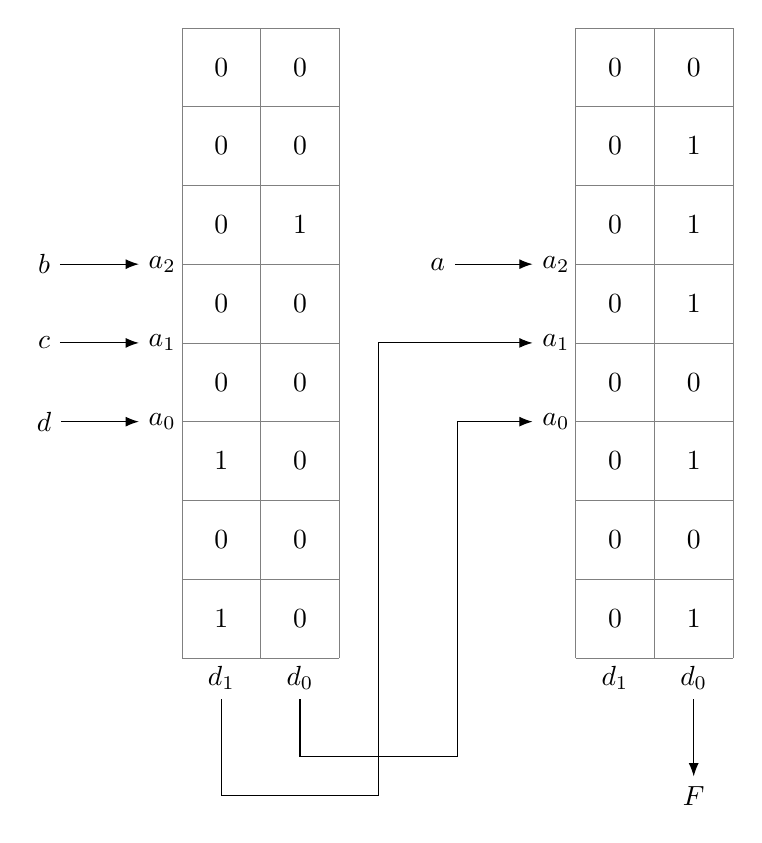
\begin{tikzpicture}[>/.tip={Latex}]
\draw[help lines] (0,0) grid (2,8);
\foreach \i/\j in {0/0,1/0,2/0,3/0,4/0,5/1,6/0,7/1}
	\draw (0.5,7.5-\i) node {\j};
\foreach \i/\j in {0/0,1/0,2/1,3/0,4/0,5/0,6/0,7/0}
	\draw (1.5,7.5-\i) node {\j};
\draw (-0.25,5) node (a2) {$a_2$};
\draw (-0.25,4) node (a1) {$a_1$};
\draw (-0.25,3) node (a0) {$a_0$};
\draw (a2)++(left:1.5cm) node (b) {$b$};
\draw (a1)++(left:1.5cm) node (c) {$c$};
\draw (a0)++(left:1.5cm) node (d) {$d$};
\draw[->] (b) -- (a2);
\draw[->] (c) -- (a1);
\draw[->] (d) -- (a0);
\draw (0.5,-0.25) node (d1) {$d_1$};
\draw (1.5,-0.25) node (d0) {$d_0$};

\draw[help lines] (5,0) grid (7,8);
\foreach \i/\j in {0/0,1/0,2/0,3/0,4/0,5/0,6/0,7/0}
	\draw (5.5,7.5-\i) node {\j};
\foreach \i/\j in {0/0,1/1,2/1,3/1,4/0,5/1,6/0,7/1}
	\draw (6.5,7.5-\i) node {\j};
\draw (5-0.25,5) node (a2) {$a_2$};
\draw (5-0.25,4) node (a1) {$a_1$};
\draw (5-0.25,3) node (a0) {$a_0$};
\draw (a2)++(left:1.5cm) node (a) {$a$};
\draw[->] (a) -- (a2);
\draw[->] (d1) -- ++(down:1.5cm) -- ++(right:2cm) |- (a1);
\draw[->] (d0) -- ++(down:1cm) -- ++(right:2cm) |- (a0);
\draw (5.5,-0.25) node (d1) {$d_1$};
\draw (6.5,-0.25) node (d0) {$d_0$};
\draw (d0)++(down:1.5cm) node (F) {$F$};
\draw[->] (d0) -- (F);
\end{tikzpicture}
\end{center}

\section{}

\begin{center}
\begin{tikzpicture}[>/.tip={Latex}]
\draw[help lines] (0,0) grid (16,1);
\foreach \i/\j in {0/0,1/0,2/0,3/0,4/1,5/1,6/1,7/1,8/0,9/0,10/0,11/0,12/1,13/0,14/1,15/1} {
	\draw (\i+0.5,1.25) node {\i};
	\draw (\i+0.5,0.5) node {\j};
}
\foreach \i in {1,...,4} {
	\draw (\i*2+3,2.5) node (x\i) {$x_\i$};
	\draw[->] (x\i) -- (\i*2+3,1);
}
\draw (8,-1.5) node (f) {$f$};
\draw[->] (8,0) -- (f);
\end{tikzpicture}
\end{center}

\end{document}
